% Options for packages loaded elsewhere
\PassOptionsToPackage{unicode}{hyperref}
\PassOptionsToPackage{hyphens}{url}
\PassOptionsToPackage{dvipsnames,svgnames,x11names}{xcolor}
%
\documentclass[
]{article}
\usepackage{amsmath,amssymb}
\usepackage{lmodern}
\usepackage{iftex}
\ifPDFTeX
  \usepackage[T1]{fontenc}
  \usepackage[utf8]{inputenc}
  \usepackage{textcomp} % provide euro and other symbols
\else % if luatex or xetex
  \usepackage{unicode-math}
  \defaultfontfeatures{Scale=MatchLowercase}
  \defaultfontfeatures[\rmfamily]{Ligatures=TeX,Scale=1}
\fi
% Use upquote if available, for straight quotes in verbatim environments
\IfFileExists{upquote.sty}{\usepackage{upquote}}{}
\IfFileExists{microtype.sty}{% use microtype if available
  \usepackage[]{microtype}
  \UseMicrotypeSet[protrusion]{basicmath} % disable protrusion for tt fonts
}{}
\makeatletter
\@ifundefined{KOMAClassName}{% if non-KOMA class
  \IfFileExists{parskip.sty}{%
    \usepackage{parskip}
  }{% else
    \setlength{\parindent}{0pt}
    \setlength{\parskip}{6pt plus 2pt minus 1pt}}
}{% if KOMA class
  \KOMAoptions{parskip=half}}
\makeatother
\usepackage{xcolor}
\usepackage[margin=1in]{geometry}
\usepackage{color}
\usepackage{fancyvrb}
\newcommand{\VerbBar}{|}
\newcommand{\VERB}{\Verb[commandchars=\\\{\}]}
\DefineVerbatimEnvironment{Highlighting}{Verbatim}{commandchars=\\\{\}}
% Add ',fontsize=\small' for more characters per line
\usepackage{framed}
\definecolor{shadecolor}{RGB}{248,248,248}
\newenvironment{Shaded}{\begin{snugshade}}{\end{snugshade}}
\newcommand{\AlertTok}[1]{\textcolor[rgb]{0.94,0.16,0.16}{#1}}
\newcommand{\AnnotationTok}[1]{\textcolor[rgb]{0.56,0.35,0.01}{\textbf{\textit{#1}}}}
\newcommand{\AttributeTok}[1]{\textcolor[rgb]{0.77,0.63,0.00}{#1}}
\newcommand{\BaseNTok}[1]{\textcolor[rgb]{0.00,0.00,0.81}{#1}}
\newcommand{\BuiltInTok}[1]{#1}
\newcommand{\CharTok}[1]{\textcolor[rgb]{0.31,0.60,0.02}{#1}}
\newcommand{\CommentTok}[1]{\textcolor[rgb]{0.56,0.35,0.01}{\textit{#1}}}
\newcommand{\CommentVarTok}[1]{\textcolor[rgb]{0.56,0.35,0.01}{\textbf{\textit{#1}}}}
\newcommand{\ConstantTok}[1]{\textcolor[rgb]{0.00,0.00,0.00}{#1}}
\newcommand{\ControlFlowTok}[1]{\textcolor[rgb]{0.13,0.29,0.53}{\textbf{#1}}}
\newcommand{\DataTypeTok}[1]{\textcolor[rgb]{0.13,0.29,0.53}{#1}}
\newcommand{\DecValTok}[1]{\textcolor[rgb]{0.00,0.00,0.81}{#1}}
\newcommand{\DocumentationTok}[1]{\textcolor[rgb]{0.56,0.35,0.01}{\textbf{\textit{#1}}}}
\newcommand{\ErrorTok}[1]{\textcolor[rgb]{0.64,0.00,0.00}{\textbf{#1}}}
\newcommand{\ExtensionTok}[1]{#1}
\newcommand{\FloatTok}[1]{\textcolor[rgb]{0.00,0.00,0.81}{#1}}
\newcommand{\FunctionTok}[1]{\textcolor[rgb]{0.00,0.00,0.00}{#1}}
\newcommand{\ImportTok}[1]{#1}
\newcommand{\InformationTok}[1]{\textcolor[rgb]{0.56,0.35,0.01}{\textbf{\textit{#1}}}}
\newcommand{\KeywordTok}[1]{\textcolor[rgb]{0.13,0.29,0.53}{\textbf{#1}}}
\newcommand{\NormalTok}[1]{#1}
\newcommand{\OperatorTok}[1]{\textcolor[rgb]{0.81,0.36,0.00}{\textbf{#1}}}
\newcommand{\OtherTok}[1]{\textcolor[rgb]{0.56,0.35,0.01}{#1}}
\newcommand{\PreprocessorTok}[1]{\textcolor[rgb]{0.56,0.35,0.01}{\textit{#1}}}
\newcommand{\RegionMarkerTok}[1]{#1}
\newcommand{\SpecialCharTok}[1]{\textcolor[rgb]{0.00,0.00,0.00}{#1}}
\newcommand{\SpecialStringTok}[1]{\textcolor[rgb]{0.31,0.60,0.02}{#1}}
\newcommand{\StringTok}[1]{\textcolor[rgb]{0.31,0.60,0.02}{#1}}
\newcommand{\VariableTok}[1]{\textcolor[rgb]{0.00,0.00,0.00}{#1}}
\newcommand{\VerbatimStringTok}[1]{\textcolor[rgb]{0.31,0.60,0.02}{#1}}
\newcommand{\WarningTok}[1]{\textcolor[rgb]{0.56,0.35,0.01}{\textbf{\textit{#1}}}}
\usepackage{graphicx}
\makeatletter
\def\maxwidth{\ifdim\Gin@nat@width>\linewidth\linewidth\else\Gin@nat@width\fi}
\def\maxheight{\ifdim\Gin@nat@height>\textheight\textheight\else\Gin@nat@height\fi}
\makeatother
% Scale images if necessary, so that they will not overflow the page
% margins by default, and it is still possible to overwrite the defaults
% using explicit options in \includegraphics[width, height, ...]{}
\setkeys{Gin}{width=\maxwidth,height=\maxheight,keepaspectratio}
% Set default figure placement to htbp
\makeatletter
\def\fps@figure{htbp}
\makeatother
\setlength{\emergencystretch}{3em} % prevent overfull lines
\providecommand{\tightlist}{%
  \setlength{\itemsep}{0pt}\setlength{\parskip}{0pt}}
\setcounter{secnumdepth}{-\maxdimen} % remove section numbering
\ifLuaTeX
  \usepackage{selnolig}  % disable illegal ligatures
\fi
\IfFileExists{bookmark.sty}{\usepackage{bookmark}}{\usepackage{hyperref}}
\IfFileExists{xurl.sty}{\usepackage{xurl}}{} % add URL line breaks if available
\urlstyle{same} % disable monospaced font for URLs
\hypersetup{
  pdftitle={BDA - Project},
  pdfauthor={Anonymous},
  colorlinks=true,
  linkcolor={Maroon},
  filecolor={Maroon},
  citecolor={Blue},
  urlcolor={blue},
  pdfcreator={LaTeX via pandoc}}

\title{BDA - Project}
\author{Anonymous}
\date{}

\begin{document}
\maketitle

{
\hypersetup{linkcolor=}
\setcounter{tocdepth}{1}
\tableofcontents
}
\hypertarget{introduction}{%
\section{Introduction}\label{introduction}}

Nowadays, given the enormous amount of data that is generated, it is
essential to be able to perform precise analyzes in order to have an
important advantage over competitors. In particular, data analysis is
proving increasingly important in the world of sport and currently most
of high-level teams rely on data scientists. In this report, we will
focus on the MotoGP sport which is the premier class of motorcycle road
racing events held on road circuits. Using a public data-set of the
MotoGP results from 2012 to 2021, we designed two different models to
describe how drivers and constructions can affect the result of the
final world champion. We were curious to understand what is more
relevant between drivers and construction teams and whether the chances
of final victory for ordinary drivers with first-class teams are higher
than normal teams with champion drivers. The first model takes into
account only the drivers and construction teams but the results were not
satisfactory. Indeed, we found out that the performance of the
motorbikes differ according to the technological development and the
same motorbike can have opposite performances from year to year. That
said, in the second model we introduced the year variable and thus the
results have improved significantly.

\hypertarget{data}{%
\section{Data}\label{data}}

The dataset used is public on the website at this
\href{https://observablehq.com/@piratus/motogp-results-database}{link}.
It is an SQLite database with MotoGP race results and it contains 15
tables: bikes, categories, circuits, countries, gp\_country\_codes,
race\_conditions, race\_results, races, riders, season\_categories,
season\_results, seasons, stage\_names, stages, and teams. By using a
JavaScript script, we downloaded the table race\_results\_view where
each row represents the finish position of a driver for a specific race.
The fields that interest us are: (a) year: race year. (b) sequence: race
number for a specific year. Every first race of every year has sequence
equal to 1, the second race has sequence equal to 2 and so on. (c)
rider\_name: name of the drive. (d) team\_name: name of the construction
team. (e) position: final position for a specific driver in a specific
race.

\hypertarget{data-preparation}{%
\subsection{Data Preparation}\label{data-preparation}}

\hypertarget{some-eda--}{%
\subsection{Some EDA ----}\label{some-eda--}}

\begin{Shaded}
\begin{Highlighting}[]
\NormalTok{data }\OtherTok{=} \FunctionTok{read.csv}\NormalTok{(}\StringTok{"./data/race\_results\_view.csv"}\NormalTok{)}
\end{Highlighting}
\end{Shaded}

\begin{Shaded}
\begin{Highlighting}[]
\CommentTok{\# Data processing }
\DocumentationTok{\#\# Restricting my analysis to the period 2012{-}2021}
\NormalTok{data }\OtherTok{\textless{}{-}}\NormalTok{ data }\SpecialCharTok{\%\textgreater{}\%} \FunctionTok{filter}\NormalTok{(}
\NormalTok{  position }\SpecialCharTok{\textgreater{}} \DecValTok{0}\NormalTok{,}
\NormalTok{  year }\SpecialCharTok{\textgreater{}} \DecValTok{2011}
\NormalTok{)}
\DocumentationTok{\#\# convert to factors}
\NormalTok{data }\OtherTok{\textless{}{-}}\NormalTok{ data }\SpecialCharTok{\%\textgreater{}\%} \FunctionTok{mutate}\NormalTok{(}
  \AttributeTok{rider\_name  =} \FunctionTok{as.factor}\NormalTok{(rider\_name),}
  \AttributeTok{team\_name  =} \FunctionTok{as.factor}\NormalTok{(team\_name)}
\NormalTok{)}

\CommentTok{\# New variables}
\NormalTok{data }\OtherTok{\textless{}{-}}\NormalTok{ data }\SpecialCharTok{\%\textgreater{}\%} \FunctionTok{group\_by}\NormalTok{(year, sequence) }\SpecialCharTok{\%\textgreater{}\%} \FunctionTok{mutate}\NormalTok{(  }
  \AttributeTok{position\_prop =}\NormalTok{ (}\FunctionTok{n}\NormalTok{() }\SpecialCharTok{{-}}\NormalTok{ position) }\SpecialCharTok{/}\NormalTok{ (}\FunctionTok{n}\NormalTok{() }\SpecialCharTok{{-}} \DecValTok{1}\NormalTok{),        }
  \AttributeTok{prop\_trans =}\NormalTok{ (position\_prop }\SpecialCharTok{*}\NormalTok{ (}\FunctionTok{n}\NormalTok{() }\SpecialCharTok{{-}} \DecValTok{1}\NormalTok{) }\SpecialCharTok{+} \FloatTok{0.5}\NormalTok{) }\SpecialCharTok{/} \FunctionTok{n}\NormalTok{() }
\NormalTok{  )}

\NormalTok{data }\OtherTok{\textless{}{-}}\NormalTok{ data }\SpecialCharTok{\%\textgreater{}\%} 
  \FunctionTok{mutate}\NormalTok{(}
    \AttributeTok{team\_name =} \FunctionTok{case\_when}\NormalTok{(team\_name }\SpecialCharTok{==} \StringTok{"Movistar Yamaha MotoGP"} \SpecialCharTok{\textasciitilde{}} \StringTok{"Yamaha MotoGP"}\NormalTok{,}
\NormalTok{                          team\_name }\SpecialCharTok{==} \StringTok{"Monster Energy Yamaha MotoGP"} \SpecialCharTok{\textasciitilde{}} \StringTok{"Yamaha MotoGP"}\NormalTok{,}
\NormalTok{                          team\_name }\SpecialCharTok{==} \StringTok{"Yamaha Factory Racing"} \SpecialCharTok{\textasciitilde{}} \StringTok{"Yamaha MotoGP"}\NormalTok{,}
                          \ConstantTok{TRUE} \SpecialCharTok{\textasciitilde{}} \FunctionTok{as.character}\NormalTok{(team\_name))}
\NormalTok{  )}
\end{Highlighting}
\end{Shaded}

The variable position\_prop represents how many rider\_names you beat in
a race, the variables position\_trans is a transformation: Indeed The
documentation for the R betareg package mentions that: ``if y also
assumes the extremes 0 and 1, a useful transformation in practice is (y
* (n-1) + 0.5) / n where n is the sample size''.

(see \url{https://stats.stackexchange.com/a/134297/116878})

Preliminary plots

\begin{Shaded}
\begin{Highlighting}[]
\DocumentationTok{\#\# finish position}
\FunctionTok{ggplot}\NormalTok{(data, }\FunctionTok{aes}\NormalTok{(}\AttributeTok{x =} \FunctionTok{factor}\NormalTok{(position))) }\SpecialCharTok{+}
  \FunctionTok{geom\_bar}\NormalTok{(}\AttributeTok{fill =} \StringTok{"darkmagenta"}\NormalTok{) }\SpecialCharTok{+}
  \FunctionTok{labs}\NormalTok{(}
    \AttributeTok{title =} \StringTok{"Distribution of finish positions"}\NormalTok{,}
    \AttributeTok{subtitle =} \StringTok{"Era (2012{-}2021)"}\NormalTok{,}
    \AttributeTok{x =} \StringTok{"Finish position"}\NormalTok{,}
    \AttributeTok{y =} \StringTok{"Count"}
\NormalTok{  )}
\end{Highlighting}
\end{Shaded}

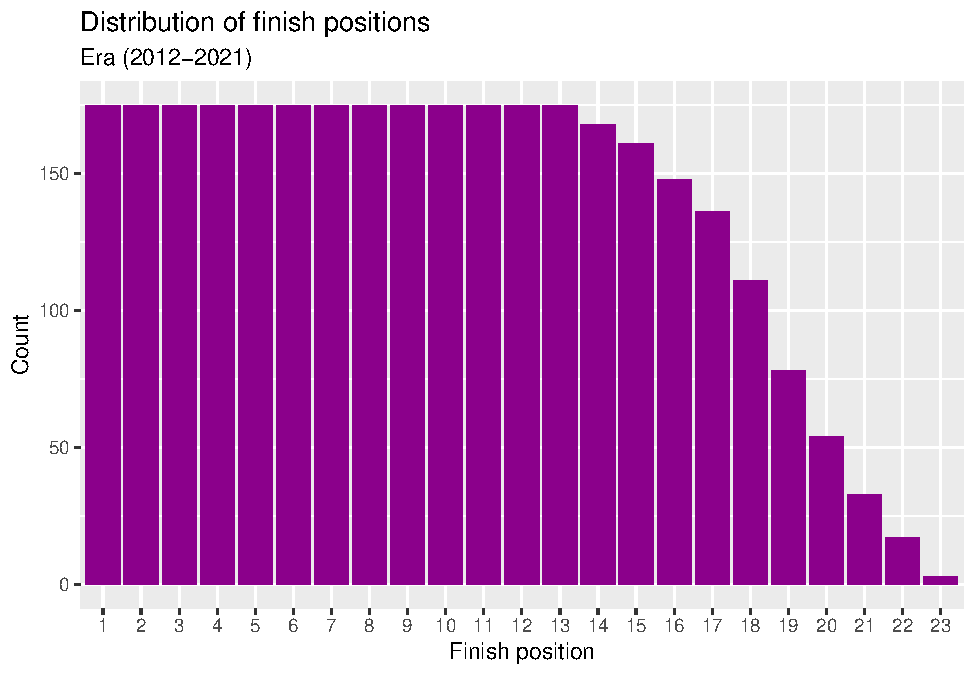
\includegraphics{Project_files/figure-latex/unnamed-chunk-4-1.pdf}

\begin{Shaded}
\begin{Highlighting}[]
\NormalTok{data }\SpecialCharTok{\%\textgreater{}\%}
  \FunctionTok{filter}\NormalTok{(rider\_name }\SpecialCharTok{\%in\%} \FunctionTok{c}\NormalTok{(}\StringTok{"Rossi, Valentino"}\NormalTok{, }\StringTok{"Quartararo, Fabio"}\NormalTok{, }\StringTok{"Marquez, Marc"}\NormalTok{, }\StringTok{"Lorenzo, Jorge"}\NormalTok{)) }\SpecialCharTok{\%\textgreater{}\%}
  \FunctionTok{ggplot}\NormalTok{(}\FunctionTok{aes}\NormalTok{(}\AttributeTok{x =} \FunctionTok{factor}\NormalTok{(position), }\AttributeTok{fill =}\NormalTok{ rider\_name)) }\SpecialCharTok{+}
  \FunctionTok{geom\_bar}\NormalTok{(}\AttributeTok{position =} \FunctionTok{position\_dodge}\NormalTok{(}\AttributeTok{preserve =} \StringTok{"single"}\NormalTok{)) }\SpecialCharTok{+}
  \FunctionTok{scale\_x\_discrete}\NormalTok{(}\AttributeTok{limits=}\NormalTok{rev,}\AttributeTok{breaks=}\FunctionTok{seq}\NormalTok{(}\DecValTok{1}\NormalTok{, }\DecValTok{23}\NormalTok{, }\DecValTok{3}\NormalTok{)) }\SpecialCharTok{+}
  \FunctionTok{labs}\NormalTok{(}
    \AttributeTok{x =} \StringTok{"Finish position"}\NormalTok{,}
    \AttributeTok{y =} \StringTok{"Count"}\NormalTok{,}
    \AttributeTok{title =} \StringTok{"Different rider\textquotesingle{}s finish positions"}\NormalTok{,}
    \AttributeTok{subtitle =} \StringTok{"Conditional on finishing the race"}\NormalTok{,}
    \AttributeTok{fill =} \StringTok{""}
\NormalTok{  ) }\SpecialCharTok{+}
  \FunctionTok{theme}\NormalTok{(}\AttributeTok{legend.position =} \StringTok{"top"}\NormalTok{) }\SpecialCharTok{+}
  \FunctionTok{facet\_wrap}\NormalTok{(}\SpecialCharTok{\textasciitilde{}}\NormalTok{year)}
\end{Highlighting}
\end{Shaded}

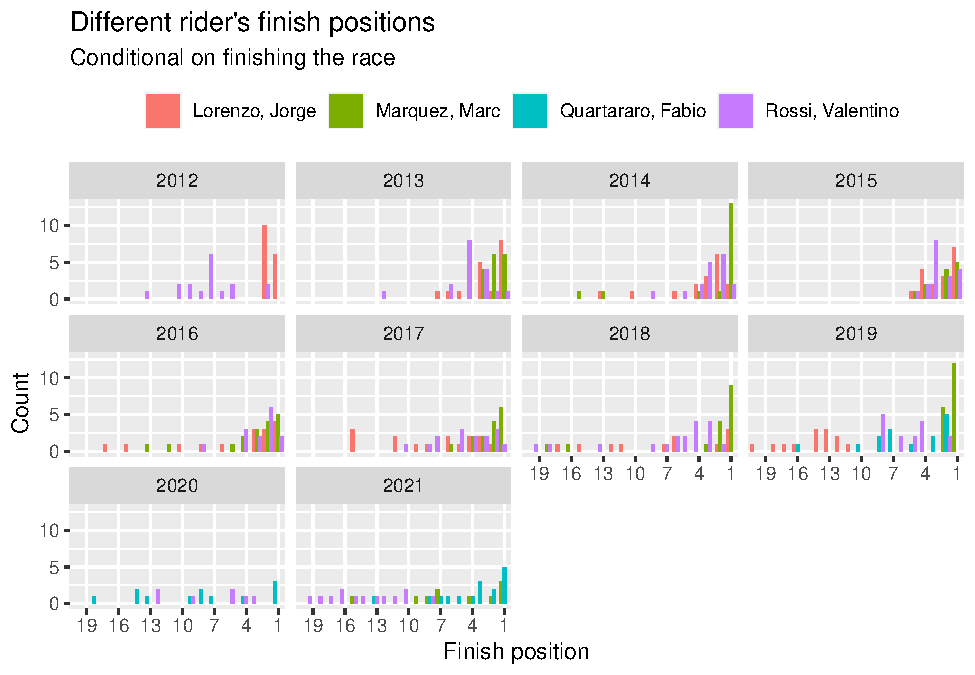
\includegraphics{Project_files/figure-latex/unnamed-chunk-5-1.pdf} Dire
che non tutti i piloti sono sempre presenti (alcuni si ritirano, altri
arrivano dopo)

\begin{Shaded}
\begin{Highlighting}[]
\NormalTok{data }\SpecialCharTok{\%\textgreater{}\%}
  \FunctionTok{filter}\NormalTok{(rider\_name }\SpecialCharTok{\%in\%} \FunctionTok{c}\NormalTok{(}\StringTok{"Rossi, Valentino"}\NormalTok{, }\StringTok{"Crutchlow, Cal"}\NormalTok{, }\StringTok{"Marquez, Marc"}\NormalTok{)) }\SpecialCharTok{\%\textgreater{}\%}
  \FunctionTok{ggplot}\NormalTok{(}\FunctionTok{aes}\NormalTok{(}\AttributeTok{x =}\NormalTok{ prop\_trans, }\AttributeTok{fill =}\NormalTok{ rider\_name)) }\SpecialCharTok{+}
  \FunctionTok{geom\_density}\NormalTok{(}\AttributeTok{alpha =} \FloatTok{0.5}\NormalTok{, }\AttributeTok{bw =} \FloatTok{0.1}\NormalTok{) }\SpecialCharTok{+}
  \FunctionTok{labs}\NormalTok{(}
    \AttributeTok{x =} \StringTok{"Smoothed proportion of outperformed rider\_names"}\NormalTok{,}
    \AttributeTok{y =} \StringTok{"Density"}\NormalTok{,}
    \AttributeTok{title =} \StringTok{"Different rider\_names\textquotesingle{} results"}\NormalTok{,}
    \AttributeTok{subtitle =} \StringTok{"Proportion of finished drivers outperformed"}\NormalTok{,}
    \AttributeTok{fill =} \StringTok{""}
\NormalTok{  ) }\SpecialCharTok{+}
  \FunctionTok{theme}\NormalTok{(}\AttributeTok{legend.position =} \StringTok{"top"}\NormalTok{, }\AttributeTok{axis.text.x =} \FunctionTok{element\_text}\NormalTok{(}\AttributeTok{angle =} \DecValTok{45}\NormalTok{, }\AttributeTok{vjust =} \FloatTok{0.85}\NormalTok{)) }\SpecialCharTok{+}
  \FunctionTok{facet\_wrap}\NormalTok{(}\SpecialCharTok{\textasciitilde{}}\NormalTok{year)}
\end{Highlighting}
\end{Shaded}

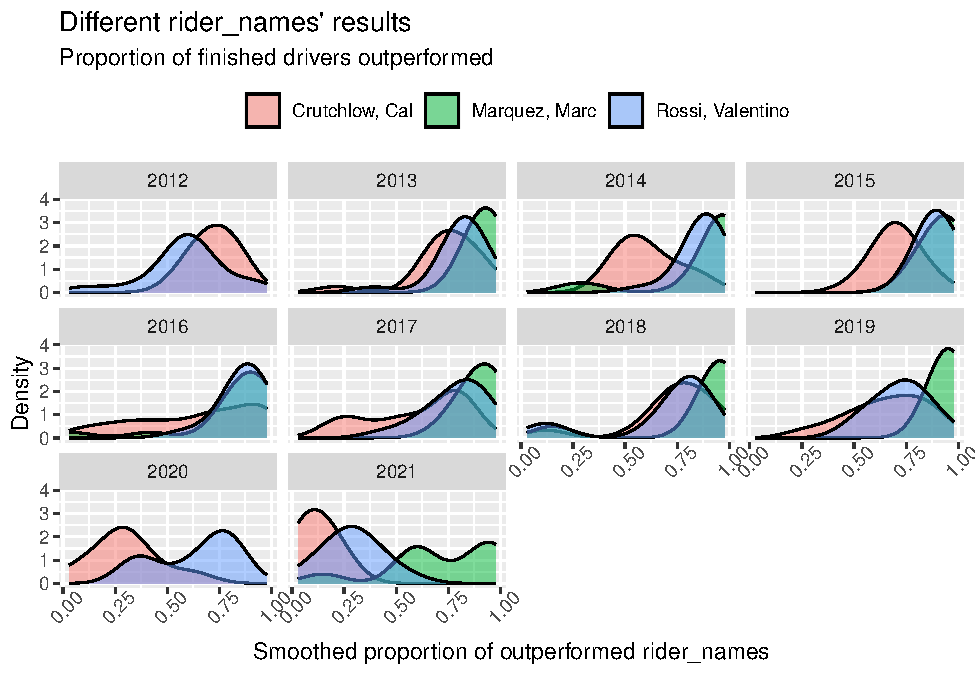
\includegraphics{Project_files/figure-latex/unnamed-chunk-6-1.pdf}

\hypertarget{description-of-the-models}{%
\section{Description of the models}\label{description-of-the-models}}

spiegare cosa rappresentano i vari beta

For driver d and constructor c , we specify the following generative
multilevel model for the proportion of drivers beaten \(y_{dc}\):

\[\begin{align*} y_{dc} \sim {\sf Beta}(\mu_{dc},\Phi) \\ logit(\mu_{dc}) = \beta_{d}  + \beta_{c}  \\ \beta_{d} \sim {\mathcal N}(0,\sigma^{2}_{d}) \\  \beta_{c} \sim {\mathcal N}(0,\sigma^{2}_{c}) \\ \sigma_{d} \sim {\mathcal \Gamma}(1,1) \\ \sigma_{c} \sim {\mathcal \Gamma}(1,1) \\ \Phi \sim \Gamma(1,1) \end{align*}\]

The Beta distribution of the model does not follow the standard
\((\alpha,\beta)\) parametrization, but rather a Beta regression
formulation with a mean parameter \(\mu\) and a dispersion parameter
\(\Phi\) (Ferrari and Cribari-Neto, 2004).

In particular, for regression analysis it is useful to model the mean of
the response. Also it is typical to define the model so that it contains
a precision (dispersion) parameter. In order to do that we can define
\[\mu = \frac{\alpha}{\alpha+\beta}\] and \[\Phi = \alpha + \beta\] so
that \[E(y) = \mu\] and \[var(y) = \frac{\mu(1-\mu)}{1+\Phi}\]. such
that \(\mu\) is the mean of the response variable and \(\Phi\) can be
interpreted as a precision parameter

The (hypothetical) average driver at an average team will on average
have \(\mu_{dc}\) = 0, which translates into a probability of 0.5 of
beating other drivers.

Then, \(\beta_{d}\) represents the mean driver skill as a log-odds
ratio; e.g., if \(\beta_{d}\) = 0,3, this means that the probability of
beating other drivers is \(\frac{1}{1 + e^{-0.3}} \simeq 0.57\)

Taking into account that the performances of a driver can change over
years (e.g.~for his age or for his experience), and that also the
quality of the motorbike can depends on the season (e.g.~for new
technologies) \(y_{dcs}\):

\[\begin{align*} y_{dcs} \sim {\mathcal Beta}(\mu_{dcs},\Phi) \\ logit(\mu_{dcs}) = \beta_{d} + \beta_{ds} + \beta_{c} + \beta_{cs} \\ \beta_{d} \sim {\mathcal N}(0,\sigma^{2}_{d}) \\ \beta_{ds} \sim {\mathcal N}(0,\sigma^{2}_{ds}) \\ \beta_{c} \sim {\mathcal N}(0,\sigma^{2}_{c}) \\ \beta_{cs} \sim {\mathcal N}(0,\sigma^{2}_{cs}) \\ \sigma_{d} \sim {\mathcal \Gamma}(1,1) \\ \sigma_{ds} \sim {\mathcal \Gamma}(1,1) \\ \sigma_{c} \sim {\mathcal \Gamma}(1,1) \\ \sigma_{cs} \sim {\mathcal \Gamma}(1,1) \\ \Phi \sim \Gamma(1,1) \end{align*}\]

So here we also included the seasonal driver form parameter
\(\beta_{ds}\), which represents yearly deviations from the long-term
average driver skill and \(\beta_{cs}\), which represents yearly
deviations from the long-term average constructor advantage.

\hypertarget{priors}{%
\subsection{Priors}\label{priors}}

We choose a weakly informative for the \(\Phi\) parameters and weakly
informative hyperpriors for the \(\sigma\) parameters in both the
models. Indeed a \(\Gamma(1,1)\) is a common choice, since it is a
distribution that starting from 0 start decreasing with a ``Gaussian
like trend'': it behaves similar to the right tail of a Gaussian or a
Cauchy centered in 0.

\begin{verbatim}
list_drivers = list(y_riders = driver_prop, N = nrow(driver_prop), J_riders = ncol(driver_prop))
# fit_driver <- hierarchical_model_d$sample(data = list_drivers, refresh=1000)
\end{verbatim}

\begin{verbatim}
prior <- c(
    prior(gamma(1,1), class = sd),
    prior(gamma(1,1), class = phi)
   )
# basic model
fit_basic <- brm(
  formula = prop_trans ~ 0 + (1 | rider_name) + (1 | team_name),
  family  = Beta(),
  data    = data,
  prior = prior,
  backend = "cmdstanr",
  chains  = 4,
  cores   = 6,
  threads = 3,
  warmup  = 1000,
  iter    = 3500
)
write_rds(fit_basic, "./fit/fit_basic.rds")
\end{verbatim}

\begin{Shaded}
\begin{Highlighting}[]
\NormalTok{fit\_basic }\OtherTok{=} \FunctionTok{readRDS}\NormalTok{(}\StringTok{"./fit/fit\_basic.rds"}\NormalTok{) }\SpecialCharTok{\%\textgreater{}\%} \FunctionTok{add\_criterion}\NormalTok{(}\StringTok{"loo"}\NormalTok{)}
\end{Highlighting}
\end{Shaded}

\begin{verbatim}
## Warning: Found 13 observations with a pareto_k > 0.7 in model '.'. It is
## recommended to set 'moment_match = TRUE' in order to perform moment matching for
## problematic observations.
\end{verbatim}

\begin{Shaded}
\begin{Highlighting}[]
\FunctionTok{summary}\NormalTok{(fit\_basic)}
\end{Highlighting}
\end{Shaded}

\begin{verbatim}
##  Family: beta 
##   Links: mu = logit; phi = identity 
## Formula: prop_trans ~ 0 + (1 | rider_name) + (1 | team_name) 
##    Data: data (Number of observations: 3184) 
##   Draws: 4 chains, each with iter = 3500; warmup = 1000; thin = 1;
##          total post-warmup draws = 10000
## 
## Group-Level Effects: 
## ~rider_name (Number of levels: 89) 
##               Estimate Est.Error l-95% CI u-95% CI Rhat Bulk_ESS Tail_ESS
## sd(Intercept)     1.06      0.11     0.87     1.30 1.00     1548     2773
## 
## ~team_name (Number of levels: 72) 
##               Estimate Est.Error l-95% CI u-95% CI Rhat Bulk_ESS Tail_ESS
## sd(Intercept)     0.57      0.07     0.44     0.72 1.00     2138     4377
## 
## Family Specific Parameters: 
##     Estimate Est.Error l-95% CI u-95% CI Rhat Bulk_ESS Tail_ESS
## phi     4.81      0.12     4.58     5.04 1.00    18690     7103
## 
## Draws were sampled using sample(hmc). For each parameter, Bulk_ESS
## and Tail_ESS are effective sample size measures, and Rhat is the potential
## scale reduction factor on split chains (at convergence, Rhat = 1).
\end{verbatim}

\begin{verbatim}
# year model
fit_year <- brm(
  formula = prop_trans ~ 0 + (1 | rider_name) + (1 | team_name) + (1 | rider_name:year) + (1|team_name:year),
  family  = Beta(),
  prior = prior,
  data    = data,
  backend = "cmdstanr",
  chains  = 4,
  cores   = 6,
  threads = 2,
  warmup  = 1000,
  iter    = 3500
)
write_rds(fit_year, "./fit/fit_year.rds")
\end{verbatim}

\begin{Shaded}
\begin{Highlighting}[]
\NormalTok{fit\_year }\OtherTok{=} \FunctionTok{readRDS}\NormalTok{(}\StringTok{"./fit/fit\_year.rds"}\NormalTok{) }\SpecialCharTok{\%\textgreater{}\%} \FunctionTok{add\_criterion}\NormalTok{(}\StringTok{"loo"}\NormalTok{)}
\end{Highlighting}
\end{Shaded}

\begin{verbatim}
## Warning: Found 20 observations with a pareto_k > 0.7 in model '.'. It is
## recommended to set 'moment_match = TRUE' in order to perform moment matching for
## problematic observations.
\end{verbatim}

\begin{Shaded}
\begin{Highlighting}[]
\FunctionTok{summary}\NormalTok{(fit\_year)}
\end{Highlighting}
\end{Shaded}

\begin{verbatim}
##  Family: beta 
##   Links: mu = logit; phi = identity 
## Formula: prop_trans ~ 0 + (1 | rider_name) + (1 | team_name) + (1 | rider_name:year) + (1 | team_name:year) 
##    Data: data (Number of observations: 3184) 
##   Draws: 4 chains, each with iter = 3500; warmup = 1000; thin = 1;
##          total post-warmup draws = 10000
## 
## Group-Level Effects: 
## ~rider_name (Number of levels: 89) 
##               Estimate Est.Error l-95% CI u-95% CI Rhat Bulk_ESS Tail_ESS
## sd(Intercept)     0.99      0.13     0.76     1.26 1.00     3818     4916
## 
## ~rider_name:year (Number of levels: 298) 
##               Estimate Est.Error l-95% CI u-95% CI Rhat Bulk_ESS Tail_ESS
## sd(Intercept)     0.45      0.05     0.36     0.55 1.00     2004     4189
## 
## ~team_name (Number of levels: 72) 
##               Estimate Est.Error l-95% CI u-95% CI Rhat Bulk_ESS Tail_ESS
## sd(Intercept)     0.45      0.09     0.30     0.64 1.00     3946     5976
## 
## ~team_name:year (Number of levels: 158) 
##               Estimate Est.Error l-95% CI u-95% CI Rhat Bulk_ESS Tail_ESS
## sd(Intercept)     0.27      0.08     0.09     0.41 1.00     1115      959
## 
## Family Specific Parameters: 
##     Estimate Est.Error l-95% CI u-95% CI Rhat Bulk_ESS Tail_ESS
## phi     5.94      0.15     5.65     6.25 1.00    15692     7185
## 
## Draws were sampled using sample(hmc). For each parameter, Bulk_ESS
## and Tail_ESS are effective sample size measures, and Rhat is the potential
## scale reduction factor on split chains (at convergence, Rhat = 1).
\end{verbatim}

\hypertarget{rhat-convergence-diagnostics-and-interpretation}{%
\section{Rhat convergence diagnostics and
interpretation}\label{rhat-convergence-diagnostics-and-interpretation}}

Basic model

\begin{Shaded}
\begin{Highlighting}[]
\NormalTok{rhats }\OtherTok{\textless{}{-}} \FunctionTok{rhat}\NormalTok{(fit\_basic)}
\FunctionTok{any}\NormalTok{(rhats[}\SpecialCharTok{!}\FunctionTok{is.nan}\NormalTok{(rhats)] }\SpecialCharTok{\textgreater{}} \FloatTok{1.01}\NormalTok{)}
\end{Highlighting}
\end{Shaded}

\begin{verbatim}
## [1] FALSE
\end{verbatim}

Year model

\begin{Shaded}
\begin{Highlighting}[]
\NormalTok{rhats }\OtherTok{\textless{}{-}} \FunctionTok{rhat}\NormalTok{(fit\_year)}
\FunctionTok{any}\NormalTok{(rhats[}\SpecialCharTok{!}\FunctionTok{is.nan}\NormalTok{(rhats)] }\SpecialCharTok{\textgreater{}} \FloatTok{1.01}\NormalTok{)}
\end{Highlighting}
\end{Shaded}

\begin{verbatim}
## [1] FALSE
\end{verbatim}

\(\hat{R}\) is an estimate for potential scale reduction: it tell us if
we are using the correct parameters. In particular as
N-\textgreater+\(\infty\) it should decrease to 1.

Conceptually it represents the ratio between an overestimate of the
marginal posterior variance (done using a linear combination between the
within and the between variance) and the within variance.

If \(\hat{R}\) is high, then we have reason to believe that proceeding
with further simulations may improve our inference about the target
distribution of the associated scalar estimand.

A rule of thumb is that if \(\hat{R}\) \textless{} 1.01 we don't need to
increase the number of simulations, so in this case everything is fine.

\hypertarget{hmc-specific-convergence-diagnostics}{%
\section{HMC specific convergence
diagnostics}\label{hmc-specific-convergence-diagnostics}}

The HMC chains convergence can be determined by plotting the individual
chains that have been executed for the main model parameters

\begin{Shaded}
\begin{Highlighting}[]
\NormalTok{hmc\_conv }\OtherTok{\textless{}{-}} \FunctionTok{mcmc\_plot}\NormalTok{(fit\_year, }\AttributeTok{type =} \StringTok{"trace"}\NormalTok{) }\SpecialCharTok{+}
            \FunctionTok{facet\_wrap}\NormalTok{(}\SpecialCharTok{\textasciitilde{}}\NormalTok{parameter, }\AttributeTok{nrow =} \DecValTok{6}\NormalTok{, }\AttributeTok{scales =} \StringTok{"free"}\NormalTok{) }\SpecialCharTok{+}
            \FunctionTok{scale\_colour\_brewer}\NormalTok{(}\AttributeTok{type =} \StringTok{"seq"}\NormalTok{, }\AttributeTok{palette =} \StringTok{"Spectral"}\NormalTok{)}
\end{Highlighting}
\end{Shaded}

\begin{verbatim}
## No divergences to plot.
## Scale for colour is already present.
## Adding another scale for colour, which will replace the existing scale.
\end{verbatim}

\begin{Shaded}
\begin{Highlighting}[]
\NormalTok{hmc\_conv}
\end{Highlighting}
\end{Shaded}

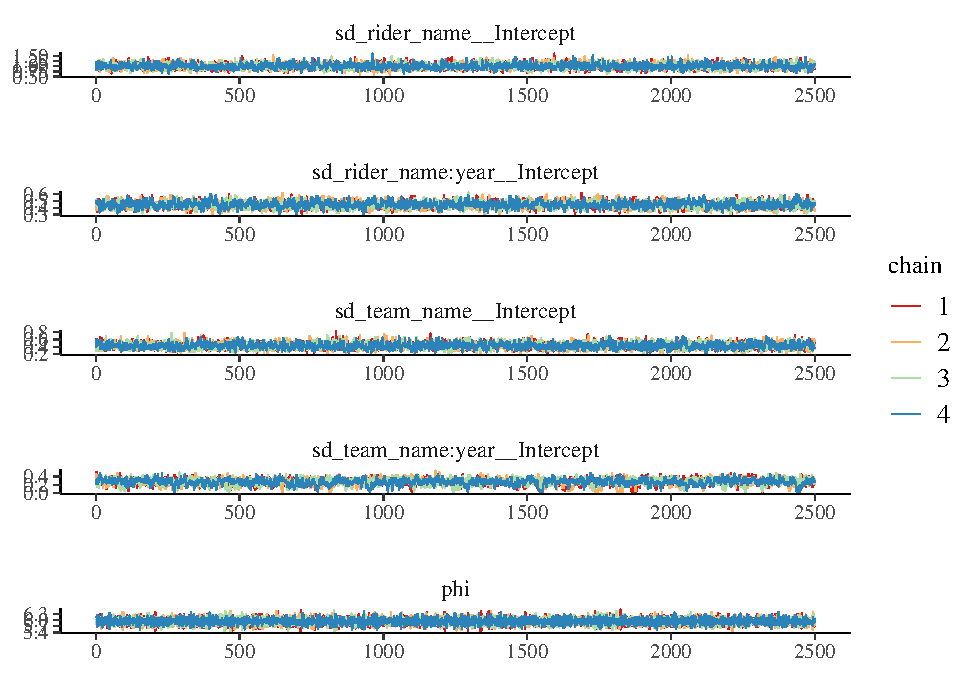
\includegraphics{Project_files/figure-latex/unnamed-chunk-11-1.pdf} By
visual inspection it can be seen how the chains for the different
parameters have converged.

\hypertarget{effective-sample-size-diagnostic-n_eff}{%
\section{Effective sample size diagnostic
(n\_eff)}\label{effective-sample-size-diagnostic-n_eff}}

\begin{Shaded}
\begin{Highlighting}[]
\FunctionTok{summary}\NormalTok{(fit\_basic)}
\end{Highlighting}
\end{Shaded}

\begin{verbatim}
##  Family: beta 
##   Links: mu = logit; phi = identity 
## Formula: prop_trans ~ 0 + (1 | rider_name) + (1 | team_name) 
##    Data: data (Number of observations: 3184) 
##   Draws: 4 chains, each with iter = 3500; warmup = 1000; thin = 1;
##          total post-warmup draws = 10000
## 
## Group-Level Effects: 
## ~rider_name (Number of levels: 89) 
##               Estimate Est.Error l-95% CI u-95% CI Rhat Bulk_ESS Tail_ESS
## sd(Intercept)     1.06      0.11     0.87     1.30 1.00     1548     2773
## 
## ~team_name (Number of levels: 72) 
##               Estimate Est.Error l-95% CI u-95% CI Rhat Bulk_ESS Tail_ESS
## sd(Intercept)     0.57      0.07     0.44     0.72 1.00     2138     4377
## 
## Family Specific Parameters: 
##     Estimate Est.Error l-95% CI u-95% CI Rhat Bulk_ESS Tail_ESS
## phi     4.81      0.12     4.58     5.04 1.00    18690     7103
## 
## Draws were sampled using sample(hmc). For each parameter, Bulk_ESS
## and Tail_ESS are effective sample size measures, and Rhat is the potential
## scale reduction factor on split chains (at convergence, Rhat = 1).
\end{verbatim}

\begin{Shaded}
\begin{Highlighting}[]
\FunctionTok{summary}\NormalTok{(fit\_year)}
\end{Highlighting}
\end{Shaded}

\begin{verbatim}
##  Family: beta 
##   Links: mu = logit; phi = identity 
## Formula: prop_trans ~ 0 + (1 | rider_name) + (1 | team_name) + (1 | rider_name:year) + (1 | team_name:year) 
##    Data: data (Number of observations: 3184) 
##   Draws: 4 chains, each with iter = 3500; warmup = 1000; thin = 1;
##          total post-warmup draws = 10000
## 
## Group-Level Effects: 
## ~rider_name (Number of levels: 89) 
##               Estimate Est.Error l-95% CI u-95% CI Rhat Bulk_ESS Tail_ESS
## sd(Intercept)     0.99      0.13     0.76     1.26 1.00     3818     4916
## 
## ~rider_name:year (Number of levels: 298) 
##               Estimate Est.Error l-95% CI u-95% CI Rhat Bulk_ESS Tail_ESS
## sd(Intercept)     0.45      0.05     0.36     0.55 1.00     2004     4189
## 
## ~team_name (Number of levels: 72) 
##               Estimate Est.Error l-95% CI u-95% CI Rhat Bulk_ESS Tail_ESS
## sd(Intercept)     0.45      0.09     0.30     0.64 1.00     3946     5976
## 
## ~team_name:year (Number of levels: 158) 
##               Estimate Est.Error l-95% CI u-95% CI Rhat Bulk_ESS Tail_ESS
## sd(Intercept)     0.27      0.08     0.09     0.41 1.00     1115      959
## 
## Family Specific Parameters: 
##     Estimate Est.Error l-95% CI u-95% CI Rhat Bulk_ESS Tail_ESS
## phi     5.94      0.15     5.65     6.25 1.00    15692     7185
## 
## Draws were sampled using sample(hmc). For each parameter, Bulk_ESS
## and Tail_ESS are effective sample size measures, and Rhat is the potential
## scale reduction factor on split chains (at convergence, Rhat = 1).
\end{verbatim}

The ess\_bulk function produces an estimated Bulk Effective Sample Size
(bulk-ESS) using rank normalized draws whereas the ess\_tail function
produces an estimated Tail Effective Sample Size (tail-ESS) by computing
the minimum of effective sample sizes for 5\% and 95\% quantiles. For
each parameter, both Bulk-ESS and Tail-ESS are bigger than 100
(approximately) per Markov Chain which means that they are reliable and
indicate that estimates of respective posterior quantiles are reliable.

\hypertarget{posterior-predictive-checking-and-interpretation}{%
\section{Posterior predictive checking and
interpretation}\label{posterior-predictive-checking-and-interpretation}}

Posterior predictive checks are an integral part of a Bayesian workflow,
where we simulate the data we expect \(\tilde{y}\) based on the model
posterior, and we compare it with the observed data \(y\), to see
whether there's consistency. Basically, if \(\tilde y\) is similar to
\(y\), then the model encapsulates the outcome well. In this case, we
decided to run the posterior predictive checks on two different years,
one in 2012 and one 2021 since there have been changes to both the rider
roaster and teams between nine years.

\begin{Shaded}
\begin{Highlighting}[]
\CommentTok{\# 2021 posterior predictive check {-}{-}{-}{-}}

\NormalTok{pred\_tab }\OtherTok{\textless{}{-}}
\NormalTok{  data }\SpecialCharTok{\%\textgreater{}\%}
  \FunctionTok{filter}\NormalTok{(year }\SpecialCharTok{==} \DecValTok{2021}\NormalTok{) }\SpecialCharTok{\%\textgreater{}\%}
  \FunctionTok{filter}\NormalTok{(}\SpecialCharTok{!}\NormalTok{(rider\_name }\SpecialCharTok{\%in\%} \FunctionTok{c}\NormalTok{(}\StringTok{"Pedrosa, Dani"}\NormalTok{,}\StringTok{"Gerloff, Garrett"}\NormalTok{,}\StringTok{"Dixon, Jake"}\NormalTok{))) }\SpecialCharTok{\%\textgreater{}\%} 
  \FunctionTok{select}\NormalTok{(rider\_name, team\_name, year)}
\end{Highlighting}
\end{Shaded}

\begin{verbatim}
## Adding missing grouping variables: `sequence`
\end{verbatim}

\begin{Shaded}
\begin{Highlighting}[]
\CommentTok{\# predict proportion of outperformed drivers}
\NormalTok{pp\_tab }\OtherTok{\textless{}{-}} \FunctionTok{posterior\_predict}\NormalTok{(fit\_year, pred\_tab)}

\DocumentationTok{\#\# Proportion plot {-}{-}{-}{-}}
\CommentTok{\# yrep}
\NormalTok{pred\_tab\_long }\OtherTok{\textless{}{-}}
\NormalTok{  pred\_tab }\SpecialCharTok{\%\textgreater{}\%}
  \FunctionTok{bind\_cols}\NormalTok{(}\FunctionTok{t}\NormalTok{(pp\_tab) }\SpecialCharTok{\%\textgreater{}\%} \FunctionTok{as\_tibble}\NormalTok{(}\AttributeTok{.name\_repair =} \StringTok{"minimal"}\NormalTok{) }\SpecialCharTok{\%\textgreater{}\%} 
  \FunctionTok{set\_names}\NormalTok{(}\DecValTok{1}\SpecialCharTok{:}\DecValTok{10000}\NormalTok{)) }\SpecialCharTok{\%\textgreater{}\%}
  \FunctionTok{pivot\_longer}\NormalTok{(}
    \AttributeTok{cols      =} \FunctionTok{c}\NormalTok{(}\SpecialCharTok{{-}}\NormalTok{rider\_name, }\SpecialCharTok{{-}}\NormalTok{team\_name, }\SpecialCharTok{{-}}\NormalTok{year),}
    \AttributeTok{names\_to  =} \StringTok{"sample"}\NormalTok{,}
    \AttributeTok{values\_to =} \StringTok{"prop\_trans"}
\NormalTok{  ) }\SpecialCharTok{\%\textgreater{}\%}
  \FunctionTok{mutate}\NormalTok{(}\AttributeTok{origin =} \StringTok{"simulated"}\NormalTok{)}

\CommentTok{\# y}
\NormalTok{true\_tab\_long }\OtherTok{\textless{}{-}}
\NormalTok{  data }\SpecialCharTok{\%\textgreater{}\%}
  \FunctionTok{filter}\NormalTok{(year }\SpecialCharTok{==} \DecValTok{2021}\NormalTok{) }\SpecialCharTok{\%\textgreater{}\%}
  \FunctionTok{filter}\NormalTok{(}\SpecialCharTok{!}\NormalTok{(rider\_name }\SpecialCharTok{\%in\%} \FunctionTok{c}\NormalTok{(}\StringTok{"Pedrosa, Dani"}\NormalTok{,}\StringTok{"Gerloff, Garrett"}\NormalTok{,}\StringTok{"Dixon, Jake"}\NormalTok{)))}\SpecialCharTok{\%\textgreater{}\%} 
  \FunctionTok{select}\NormalTok{(rider\_name, team\_name, year, prop\_trans) }\SpecialCharTok{\%\textgreater{}\%}
  \FunctionTok{mutate}\NormalTok{(}\AttributeTok{origin =} \StringTok{"observed"}\NormalTok{)}
\end{Highlighting}
\end{Shaded}

\begin{verbatim}
## Adding missing grouping variables: `sequence`
\end{verbatim}

\begin{Shaded}
\begin{Highlighting}[]
\NormalTok{ordered\_levels }\OtherTok{\textless{}{-}}
\NormalTok{  true\_tab\_long }\SpecialCharTok{\%\textgreater{}\%}
  \FunctionTok{group\_by}\NormalTok{(rider\_name) }\SpecialCharTok{\%\textgreater{}\%}
  \FunctionTok{summarise}\NormalTok{(}\AttributeTok{prop =} \FunctionTok{mean}\NormalTok{(prop\_trans)) }\SpecialCharTok{\%\textgreater{}\%}
  \FunctionTok{arrange}\NormalTok{(}\SpecialCharTok{{-}}\NormalTok{prop) }\SpecialCharTok{\%\textgreater{}\%}
  \FunctionTok{pull}\NormalTok{(rider\_name) }\SpecialCharTok{\%\textgreater{}\%}
  \FunctionTok{as.character}\NormalTok{()}


\NormalTok{PPC\_2021 }\OtherTok{\textless{}{-}} \FunctionTok{bind\_rows}\NormalTok{(pred\_tab\_long, true\_tab\_long) }\SpecialCharTok{\%\textgreater{}\%}
            \FunctionTok{ggplot}\NormalTok{(}\FunctionTok{aes}\NormalTok{(}\AttributeTok{x =}\NormalTok{ prop\_trans, }\AttributeTok{fill =}\NormalTok{ origin)) }\SpecialCharTok{+}
            \FunctionTok{geom\_density}\NormalTok{(}\AttributeTok{alpha =} \FloatTok{0.8}\NormalTok{, }\AttributeTok{bw =}\NormalTok{ .}\DecValTok{07}\NormalTok{) }\SpecialCharTok{+}
            \FunctionTok{facet\_wrap}\NormalTok{(}\SpecialCharTok{\textasciitilde{}}\FunctionTok{factor}\NormalTok{(rider\_name, }\AttributeTok{levels =}\NormalTok{ ordered\_levels), }\AttributeTok{scales =} \StringTok{"free"}\NormalTok{) }\SpecialCharTok{+}
            \FunctionTok{xlim}\NormalTok{(}\DecValTok{0}\NormalTok{, }\DecValTok{1}\NormalTok{) }\SpecialCharTok{+}
            \CommentTok{\#theme\_fira() +}
            \CommentTok{\#scale\_fill\_fira() +}
            \CommentTok{\#theme(legend.position = "top") +}
            \FunctionTok{labs}\NormalTok{(}
              \AttributeTok{title =} \StringTok{"Posterior predictive check"}\NormalTok{,}
              \AttributeTok{subtitle =} \StringTok{"2021 season"}\NormalTok{,}
              \AttributeTok{x =} \StringTok{"Proportion of outperformed riders"}\NormalTok{,}
              \AttributeTok{y =} \StringTok{""}\NormalTok{,}
              \AttributeTok{fill =} \StringTok{""}
\NormalTok{            )}

\NormalTok{PPC\_2021}
\end{Highlighting}
\end{Shaded}

\begin{verbatim}
## Warning: Removed 267 rows containing non-finite values (`stat_density()`).
\end{verbatim}

\includegraphics{Project_files/figure-latex/unnamed-chunk-13-1.pdf}
Note: In the 2021 season riders Dani Pedrosa, Jake Dixon and Gerloff
Garrett participated in one race each, so they have been excluded from
the posterior predictive check.

\begin{Shaded}
\begin{Highlighting}[]
\CommentTok{\# 2012 posterior predictive check {-}{-}{-}{-}}

\NormalTok{pred\_tab }\OtherTok{\textless{}{-}}
\NormalTok{  data }\SpecialCharTok{\%\textgreater{}\%}
  \FunctionTok{filter}\NormalTok{(year }\SpecialCharTok{==} \DecValTok{2012}\NormalTok{) }\SpecialCharTok{\%\textgreater{}\%}
  \FunctionTok{filter}\NormalTok{(}\SpecialCharTok{!}\NormalTok{(rider\_name }\SpecialCharTok{\%in\%} \FunctionTok{c}\NormalTok{(}\StringTok{"Rapp, Steve"}\NormalTok{,}\StringTok{"Battaini, Franco"}\NormalTok{,}\StringTok{"Aoyama, Hiroshi"}\NormalTok{,}\StringTok{"Vermeulen, Chris"}\NormalTok{,}
                         \StringTok{"Salom, David"}\NormalTok{,}\StringTok{"Rolfo, Roberto"}\NormalTok{, }\StringTok{"Yates, Aaron"}\NormalTok{))) }\SpecialCharTok{\%\textgreater{}\%} 
  \FunctionTok{select}\NormalTok{(rider\_name, team\_name, year)}
\end{Highlighting}
\end{Shaded}

\begin{verbatim}
## Adding missing grouping variables: `sequence`
\end{verbatim}

\begin{Shaded}
\begin{Highlighting}[]
\CommentTok{\# predict proportion of outperformed drivers}
\NormalTok{pp\_tab }\OtherTok{\textless{}{-}} \FunctionTok{posterior\_predict}\NormalTok{(fit\_year, pred\_tab)}

\DocumentationTok{\#\# Proportion plot {-}{-}{-}{-}}
\CommentTok{\# yrep}
\NormalTok{pred\_tab\_long }\OtherTok{\textless{}{-}}
\NormalTok{  pred\_tab }\SpecialCharTok{\%\textgreater{}\%}
  \FunctionTok{bind\_cols}\NormalTok{(}\FunctionTok{t}\NormalTok{(pp\_tab) }\SpecialCharTok{\%\textgreater{}\%} \FunctionTok{as\_tibble}\NormalTok{(}\AttributeTok{.name\_repair =} \StringTok{"minimal"}\NormalTok{) }\SpecialCharTok{\%\textgreater{}\%} 
  \FunctionTok{set\_names}\NormalTok{(}\DecValTok{1}\SpecialCharTok{:}\DecValTok{10000}\NormalTok{)) }\SpecialCharTok{\%\textgreater{}\%}
  \FunctionTok{pivot\_longer}\NormalTok{(}
    \AttributeTok{cols      =} \FunctionTok{c}\NormalTok{(}\SpecialCharTok{{-}}\NormalTok{rider\_name, }\SpecialCharTok{{-}}\NormalTok{team\_name, }\SpecialCharTok{{-}}\NormalTok{year),}
    \AttributeTok{names\_to  =} \StringTok{"sample"}\NormalTok{,}
    \AttributeTok{values\_to =} \StringTok{"prop\_trans"}
\NormalTok{  ) }\SpecialCharTok{\%\textgreater{}\%}
  \FunctionTok{mutate}\NormalTok{(}\AttributeTok{origin =} \StringTok{"simulated"}\NormalTok{)}

\CommentTok{\# y}
\NormalTok{true\_tab\_long }\OtherTok{\textless{}{-}}
\NormalTok{  data }\SpecialCharTok{\%\textgreater{}\%}
  \FunctionTok{filter}\NormalTok{(year }\SpecialCharTok{==} \DecValTok{2012}\NormalTok{) }\SpecialCharTok{\%\textgreater{}\%}
  \FunctionTok{filter}\NormalTok{(}\SpecialCharTok{!}\NormalTok{(rider\_name }\SpecialCharTok{\%in\%}\FunctionTok{c}\NormalTok{(}\StringTok{"Rapp, Steve"}\NormalTok{,}\StringTok{"Battaini, Franco"}\NormalTok{,}\StringTok{"Aoyama, Hiroshi"}\NormalTok{,}\StringTok{"Vermeulen, Chris"}\NormalTok{,}
                         \StringTok{"Salom, David"}\NormalTok{,}\StringTok{"Rolfo, Roberto"}\NormalTok{, }\StringTok{"Yates, Aaron"}\NormalTok{))) }\SpecialCharTok{\%\textgreater{}\%} 
  \FunctionTok{select}\NormalTok{(rider\_name, team\_name, year, prop\_trans) }\SpecialCharTok{\%\textgreater{}\%}
  \FunctionTok{mutate}\NormalTok{(}\AttributeTok{origin =} \StringTok{"observed"}\NormalTok{)}
\end{Highlighting}
\end{Shaded}

\begin{verbatim}
## Adding missing grouping variables: `sequence`
\end{verbatim}

\begin{Shaded}
\begin{Highlighting}[]
\NormalTok{ordered\_levels }\OtherTok{\textless{}{-}}
\NormalTok{  true\_tab\_long }\SpecialCharTok{\%\textgreater{}\%}
  \FunctionTok{group\_by}\NormalTok{(rider\_name) }\SpecialCharTok{\%\textgreater{}\%}
  \FunctionTok{summarise}\NormalTok{(}\AttributeTok{prop =} \FunctionTok{mean}\NormalTok{(prop\_trans)) }\SpecialCharTok{\%\textgreater{}\%}
  \FunctionTok{arrange}\NormalTok{(}\SpecialCharTok{{-}}\NormalTok{prop) }\SpecialCharTok{\%\textgreater{}\%}
  \FunctionTok{pull}\NormalTok{(rider\_name) }\SpecialCharTok{\%\textgreater{}\%}
  \FunctionTok{as.character}\NormalTok{()}


\NormalTok{PPC\_2012 }\OtherTok{\textless{}{-}} \FunctionTok{bind\_rows}\NormalTok{(pred\_tab\_long, true\_tab\_long) }\SpecialCharTok{\%\textgreater{}\%}
            \FunctionTok{ggplot}\NormalTok{(}\FunctionTok{aes}\NormalTok{(}\AttributeTok{x =}\NormalTok{ prop\_trans, }\AttributeTok{fill =}\NormalTok{ origin)) }\SpecialCharTok{+}
            \FunctionTok{geom\_density}\NormalTok{(}\AttributeTok{alpha =} \FloatTok{0.8}\NormalTok{, }\AttributeTok{bw =}\NormalTok{ .}\DecValTok{07}\NormalTok{) }\SpecialCharTok{+}
            \FunctionTok{facet\_wrap}\NormalTok{(}\SpecialCharTok{\textasciitilde{}}\FunctionTok{factor}\NormalTok{(rider\_name, }\AttributeTok{levels =}\NormalTok{ ordered\_levels), }\AttributeTok{scales =} \StringTok{"free"}\NormalTok{) }\SpecialCharTok{+}
            \FunctionTok{xlim}\NormalTok{(}\DecValTok{0}\NormalTok{, }\DecValTok{1}\NormalTok{) }\SpecialCharTok{+}
            \CommentTok{\#theme\_fira() +}
            \CommentTok{\#scale\_fill\_fira() +}
            \CommentTok{\#theme(legend.position = "top") +}
            \FunctionTok{labs}\NormalTok{(}
              \AttributeTok{title =} \StringTok{"Posterior predictive check"}\NormalTok{,}
              \AttributeTok{subtitle =} \StringTok{"2012 season"}\NormalTok{,}
              \AttributeTok{x =} \StringTok{"Proportion of outperformed riders"}\NormalTok{,}
              \AttributeTok{y =} \StringTok{""}\NormalTok{,}
              \AttributeTok{fill =} \StringTok{""}
\NormalTok{            ) }\SpecialCharTok{+}
            \FunctionTok{scale\_colour\_brewer}\NormalTok{(}\AttributeTok{type =} \StringTok{"seq"}\NormalTok{, }\AttributeTok{palette =} \StringTok{"Spectral"}\NormalTok{)}

\NormalTok{PPC\_2012}
\end{Highlighting}
\end{Shaded}

\begin{verbatim}
## Warning: Removed 268 rows containing non-finite values (`stat_density()`).
\end{verbatim}

\includegraphics{Project_files/figure-latex/unnamed-chunk-14-1.pdf}
Note: in the 2012 season riders Aaron Yates, Chris Vermeulen, David
Salom, Franco Battaini, Hiroshi Aoyama, Steve Rapp \& Roberto Rolfo have
been excluded since each of them had taken part in one Grand Prix.

Both the plots show acceptable simulated values for each individual
rider. One important thing to note is that for consistent
high-performers (ex. Quartararo Fabio - 2021, Lorenzo Jorge - 2012) and
low-performers (Salvadori Lorenzo - 2021), the posterior predictive
distribution is under-dispersed, indicating a high value for \(\phi\) in
these cases. On the other hand, for riders in the midfield (Marquez Alex
- 2021, Jonathan Rea - 2012), the posterior predictive distribution
seems to be a bit over-dispersed (low value of \(\phi\)), since there is
more variation in the observed data. But it can be seen that in both
cases, the mean estimates do not seem too biased (especially in the
midfield) so, we conclude that the model fits the observed data
satisfyingly.

\hypertarget{model-comparison-and-interpretation-of-the-results}{%
\section{Model comparison and interpretation of the
results}\label{model-comparison-and-interpretation-of-the-results}}

\begin{Shaded}
\begin{Highlighting}[]
\NormalTok{loo\_results }\OtherTok{\textless{}{-}} \FunctionTok{loo\_compare}\NormalTok{(}
\NormalTok{  fit\_basic,}
\NormalTok{  fit\_year,}
  \AttributeTok{model\_names =} \FunctionTok{c}\NormalTok{(}\StringTok{"Driver + constructor"}\NormalTok{, }\StringTok{"Driver + constructor + year"}\NormalTok{)}
\NormalTok{)}

\NormalTok{loo\_results}
\end{Highlighting}
\end{Shaded}

\begin{verbatim}
##                             elpd_diff se_diff
## Driver + constructor + year    0.0       0.0 
## Driver + constructor        -245.2      27.0
\end{verbatim}

Comparing the models, the best one is the model described by drivers,
constructors and years. Models are sorted in decreasing order: the first
is the best whereas the last is the worst. The difference in ELPD
(elpd\_diff) between the two models is considerably high, this means
that the 2 models have different predictive performance. Moreover, it is
notable how taking the year into consideration leads to significantly
better results.

\hypertarget{interpretation-of-the-results}{%
\subsection{Interpretation of the
results}\label{interpretation-of-the-results}}

Since the yearly model is better according to the LOO estimate, we
proceed our inferences with it. To determine which rider is the most
skilled, we decided to make inferences for a reduced set of riders from
the 2012-2021 period (Rossi, Pedrosa, Crutchlow, Quartararo )

The model contains a parameter that indicates the seasonal form for each
of the riders, \(\beta_{rs}\), so we can project the skill trajectories
for each of them throughout the years, while taking into consideration
any advantages due to team form or any hidden parameter uncertainties.
This is done by obtaining the posterior means and the 95\% credible
intervals for \(\beta_{r} + \beta_{rs}\) on the set of riders, for each
year

\begin{Shaded}
\begin{Highlighting}[]
\NormalTok{riders\_focus }\OtherTok{\textless{}{-}} \FunctionTok{c}\NormalTok{(}\StringTok{"Rossi"}\NormalTok{,}\StringTok{"Crutchlow"}\NormalTok{,}\StringTok{"Quartararo"}\NormalTok{,}\StringTok{"Dovizioso"}\NormalTok{)}
\NormalTok{rider\_mean }\OtherTok{\textless{}{-}} \FunctionTok{as\_draws\_df}\NormalTok{(fit\_year) }\SpecialCharTok{\%\textgreater{}\%} \FunctionTok{select}\NormalTok{(}\SpecialCharTok{{-}}\NormalTok{.chain, }\SpecialCharTok{{-}}\NormalTok{.iteration) }\SpecialCharTok{\%\textgreater{}\%} \FunctionTok{select}\NormalTok{(}\FunctionTok{contains}\NormalTok{(}\StringTok{"r\_rider\_name"}\NormalTok{),.draw) }\SpecialCharTok{\%\textgreater{}\%} \FunctionTok{select}\NormalTok{(}\SpecialCharTok{{-}}\FunctionTok{contains}\NormalTok{(}\StringTok{"year"}\NormalTok{))}
\end{Highlighting}
\end{Shaded}

\begin{verbatim}
## Warning: Dropping 'draws_df' class as required metadata was removed.
\end{verbatim}

\begin{Shaded}
\begin{Highlighting}[]
\NormalTok{rider\_form }\OtherTok{\textless{}{-}} \FunctionTok{as\_draws\_df}\NormalTok{(fit\_year) }\SpecialCharTok{\%\textgreater{}\%} \FunctionTok{select}\NormalTok{(}\SpecialCharTok{{-}}\NormalTok{.chain,}\SpecialCharTok{{-}}\NormalTok{.iteration) }\SpecialCharTok{\%\textgreater{}\%} \FunctionTok{select}\NormalTok{(}\FunctionTok{contains}\NormalTok{(}\StringTok{"r\_rider\_name:year"}\NormalTok{),.draw)}
\end{Highlighting}
\end{Shaded}

\begin{verbatim}
## Warning: Dropping 'draws_df' class as required metadata was removed.
\end{verbatim}

\begin{Shaded}
\begin{Highlighting}[]
\NormalTok{rider\_mean\_long }\OtherTok{\textless{}{-}}
\NormalTok{  rider\_mean  }\SpecialCharTok{\%\textgreater{}\%}
  \FunctionTok{pivot\_longer}\NormalTok{(}\SpecialCharTok{{-}}\NormalTok{.draw, }\AttributeTok{names\_to =} \StringTok{"Rider"}\NormalTok{, }\AttributeTok{values\_to =} \StringTok{"Skill"}\NormalTok{,}
               \AttributeTok{names\_pattern =} \StringTok{"}\SpecialCharTok{\textbackslash{}\textbackslash{}}\StringTok{[(}\SpecialCharTok{\textbackslash{}\textbackslash{}}\StringTok{w\{1,10\}.*?),..*?}\SpecialCharTok{\textbackslash{}\textbackslash{}}\StringTok{]"}\NormalTok{) }\SpecialCharTok{\%\textgreater{}\%} 
  \FunctionTok{mutate}\NormalTok{(}\AttributeTok{Rider =} \FunctionTok{as.factor}\NormalTok{(Rider))}

\NormalTok{rider\_form\_long }\OtherTok{\textless{}{-}}
\NormalTok{  rider\_form }\SpecialCharTok{\%\textgreater{}\%}
  \FunctionTok{pivot\_longer}\NormalTok{(}\SpecialCharTok{{-}}\NormalTok{.draw, }\AttributeTok{names\_to =} \FunctionTok{c}\NormalTok{(}\StringTok{"Rider"}\NormalTok{, }\StringTok{"Year"}\NormalTok{), }\AttributeTok{values\_to =} \StringTok{"Form"}\NormalTok{,}
               \AttributeTok{names\_pattern =} \StringTok{"}\SpecialCharTok{\textbackslash{}\textbackslash{}}\StringTok{[(}\SpecialCharTok{\textbackslash{}\textbackslash{}}\StringTok{w\{1,10\}).*?(}\SpecialCharTok{\textbackslash{}\textbackslash{}}\StringTok{d\{1,4\}).*?,"}\NormalTok{) }\SpecialCharTok{\%\textgreater{}\%}
  \FunctionTok{mutate}\NormalTok{(}\AttributeTok{Rider =} \FunctionTok{as.factor}\NormalTok{(Rider), }\AttributeTok{Year =} \FunctionTok{as.integer}\NormalTok{(Year))}

\NormalTok{rider\_skill\_summary }\OtherTok{\textless{}{-}}
  \FunctionTok{merge}\NormalTok{(}\AttributeTok{x=}\NormalTok{rider\_form\_long, }\AttributeTok{y=}\NormalTok{rider\_mean\_long, }\AttributeTok{by =} \FunctionTok{c}\NormalTok{(}\StringTok{"Rider"}\NormalTok{,}\StringTok{".draw"}\NormalTok{)) }\SpecialCharTok{\%\textgreater{}\%}
  \FunctionTok{mutate}\NormalTok{(}\AttributeTok{skill\_yr =}\NormalTok{ Form }\SpecialCharTok{+}\NormalTok{ Skill) }\SpecialCharTok{\%\textgreater{}\%}
  \FunctionTok{group\_by}\NormalTok{(Rider, Year) }\SpecialCharTok{\%\textgreater{}\%}
  \FunctionTok{summarise}\NormalTok{(}
    \AttributeTok{est =} \FunctionTok{mean}\NormalTok{(skill\_yr),}
    \AttributeTok{lower =} \FunctionTok{quantile}\NormalTok{(skill\_yr, }\FloatTok{0.025}\NormalTok{),}
    \AttributeTok{upper =} \FunctionTok{quantile}\NormalTok{(skill\_yr, }\FloatTok{0.975}\NormalTok{),}
\NormalTok{  )}
\end{Highlighting}
\end{Shaded}

\begin{verbatim}
## `summarise()` has grouped output by 'Rider'. You can override using the
## `.groups` argument.
\end{verbatim}

\begin{Shaded}
\begin{Highlighting}[]
\NormalTok{plt\_skill\_trajectory }\OtherTok{\textless{}{-}}
\NormalTok{  rider\_skill\_summary }\SpecialCharTok{\%\textgreater{}\%}
  \FunctionTok{ungroup}\NormalTok{() }\SpecialCharTok{\%\textgreater{}\%}
  \FunctionTok{filter}\NormalTok{(Rider }\SpecialCharTok{\%in\%}\NormalTok{ riders\_focus) }\SpecialCharTok{\%\textgreater{}\%}
  \FunctionTok{mutate}\NormalTok{(}\AttributeTok{Rider =} \FunctionTok{fct\_reorder}\NormalTok{(Rider, }\SpecialCharTok{{-}}\NormalTok{est)) }\SpecialCharTok{\%\textgreater{}\%}
  \FunctionTok{ggplot}\NormalTok{(}\FunctionTok{aes}\NormalTok{(}\AttributeTok{x =}\NormalTok{ Year, }\AttributeTok{y =}\NormalTok{ est, }\AttributeTok{ymin =}\NormalTok{ lower, }\AttributeTok{ymax =}\NormalTok{ upper)) }\SpecialCharTok{+}
  \FunctionTok{geom\_ribbon}\NormalTok{(}\FunctionTok{aes}\NormalTok{(}\AttributeTok{fill =}\NormalTok{ Rider), }\AttributeTok{alpha =}\NormalTok{ .}\DecValTok{2}\NormalTok{) }\SpecialCharTok{+}
  \FunctionTok{geom\_line}\NormalTok{(}\FunctionTok{aes}\NormalTok{(}\AttributeTok{colour =}\NormalTok{ Rider)) }\SpecialCharTok{+}
  \FunctionTok{geom\_point}\NormalTok{(}\FunctionTok{aes}\NormalTok{(}\AttributeTok{colour =}\NormalTok{ Rider)) }\SpecialCharTok{+}
  \FunctionTok{scale\_fill\_fira}\NormalTok{(}\AttributeTok{guide =} \StringTok{"none"}\NormalTok{) }\SpecialCharTok{+}
  \FunctionTok{scale\_colour\_fira}\NormalTok{(}\AttributeTok{guide =} \StringTok{"none"}\NormalTok{) }\SpecialCharTok{+}
  \CommentTok{\#theme\_fira() +}
  \FunctionTok{facet\_wrap}\NormalTok{(}\SpecialCharTok{\textasciitilde{}}\NormalTok{Rider) }\SpecialCharTok{+}
  \FunctionTok{labs}\NormalTok{(}\AttributeTok{x =} \StringTok{"Season"}\NormalTok{, }\AttributeTok{y =} \StringTok{"Skill (log odds ratio)"}\NormalTok{, }\AttributeTok{title =} \StringTok{"MotoGP Rider skill trajectories"}\NormalTok{,}
       \AttributeTok{subtitle =} \StringTok{"period (2012{-}2021) Rider skill,}\SpecialCharTok{\textbackslash{}n}\StringTok{considering for yearly team advantage."}\NormalTok{)}


\NormalTok{plt\_skill\_trajectory}
\end{Highlighting}
\end{Shaded}

\includegraphics{Project_files/figure-latex/unnamed-chunk-17-1.pdf} The
figure shows slight deviations in skills during the seasons,
continue\ldots{}

A ranking based on skill can also be produced, by focusing on a single
year, which is useful to produce on the latest year available in the
dataset (2021)

\begin{Shaded}
\begin{Highlighting}[]
\NormalTok{plt\_rider\_skill\_2021 }\OtherTok{\textless{}{-}}
\NormalTok{  rider\_skill\_summary }\SpecialCharTok{\%\textgreater{}\%}
  \FunctionTok{ungroup}\NormalTok{() }\SpecialCharTok{\%\textgreater{}\%}
  \FunctionTok{filter}\NormalTok{(Year }\SpecialCharTok{==} \DecValTok{2021}\NormalTok{) }\SpecialCharTok{\%\textgreater{}\%}
  \FunctionTok{mutate}\NormalTok{(}\AttributeTok{Rider =} \FunctionTok{fct\_reorder}\NormalTok{(Rider, est)) }\SpecialCharTok{\%\textgreater{}\%}
  \FunctionTok{ggplot}\NormalTok{(}\FunctionTok{aes}\NormalTok{(}\AttributeTok{y =}\NormalTok{ Rider, }\AttributeTok{x =}\NormalTok{ est, }\AttributeTok{xmin =}\NormalTok{ lower, }\AttributeTok{xmax =}\NormalTok{ upper)) }\SpecialCharTok{+}
  \FunctionTok{geom\_pointrange}\NormalTok{(}\AttributeTok{colour =}\NormalTok{ firaCols[}\DecValTok{3}\NormalTok{]) }\SpecialCharTok{+}
  \CommentTok{\#theme\_fira() +}
  \FunctionTok{labs}\NormalTok{(}\AttributeTok{title =} \StringTok{"2021 MotoGP rider skill"}\NormalTok{,}
       \AttributeTok{subtitle =} \StringTok{"Accounting for yearly team advantage."}\NormalTok{,}
       \AttributeTok{x =} \StringTok{"Skill (log odds ratio)"}\NormalTok{,}
       \AttributeTok{y =} \StringTok{"Rider"}\NormalTok{)}

\NormalTok{plt\_rider\_skill\_2021}
\end{Highlighting}
\end{Shaded}

\includegraphics{Project_files/figure-latex/unnamed-chunk-18-1.pdf}

In the 2021 grid, based on the figure above, it can be inferred that
Quartararo is one of the most skilled drivers. The reason behind the
wide confidence interval with Marc Marquez is due to him missing the
2020 season (1 start), and some races in the 2021 season. This combined
with the fact that he has a high skill ranking due to producing
high-performance results creates this level of uncertainity around his
skill level. (Even if the inference is only on the 2021 season
\(\beta{r}\) takes into account all the seasons (? check)).

\textbf{TO ADD TEAM ADVANTAGE + COUNTERFACTUAL FOR QUARTARARO IN ANOTHER
TEAM}

To determine how much a given bike from a certain team yields, we can
compute the posterior means and the 95\% confidence intervals for
\(\beta_t\) from the model

\begin{Shaded}
\begin{Highlighting}[]
\NormalTok{team\_focus }\OtherTok{\textless{}{-}} \FunctionTok{c}\NormalTok{(}\StringTok{"Yamaha MotoGP"}\NormalTok{, }\StringTok{"Team SUZUKI ECSTAR"}\NormalTok{, }\StringTok{"Repsol Honda Team"}\NormalTok{, }\StringTok{"Red Bull KTM Factory Racing"}\NormalTok{, }\StringTok{"Aprilia Racing Team Gresini"}\NormalTok{)}

\NormalTok{team\_mean }\OtherTok{\textless{}{-}} \FunctionTok{as\_draws\_df}\NormalTok{(fit\_year) }\SpecialCharTok{\%\textgreater{}\%} \FunctionTok{select}\NormalTok{(}\SpecialCharTok{{-}}\NormalTok{.chain, }\SpecialCharTok{{-}}\NormalTok{.iteration) }\SpecialCharTok{\%\textgreater{}\%} \FunctionTok{select}\NormalTok{(}\FunctionTok{contains}\NormalTok{(}\StringTok{"r\_team\_name"}\NormalTok{),.draw) }\SpecialCharTok{\%\textgreater{}\%} \FunctionTok{select}\NormalTok{(}\SpecialCharTok{{-}}\FunctionTok{contains}\NormalTok{(}\StringTok{"year"}\NormalTok{))}
\end{Highlighting}
\end{Shaded}

\begin{verbatim}
## Warning: Dropping 'draws_df' class as required metadata was removed.
\end{verbatim}

\begin{Shaded}
\begin{Highlighting}[]
\NormalTok{team\_form }\OtherTok{\textless{}{-}} \FunctionTok{as\_draws\_df}\NormalTok{(fit\_year) }\SpecialCharTok{\%\textgreater{}\%} \FunctionTok{select}\NormalTok{(}\SpecialCharTok{{-}}\NormalTok{.chain, }\SpecialCharTok{{-}}\NormalTok{.iteration) }\SpecialCharTok{\%\textgreater{}\%} \FunctionTok{select}\NormalTok{(}\FunctionTok{contains}\NormalTok{(}\StringTok{"r\_team\_name:year"}\NormalTok{),.draw) }
\end{Highlighting}
\end{Shaded}

\begin{verbatim}
## Warning: Dropping 'draws_df' class as required metadata was removed.
\end{verbatim}

\begin{Shaded}
\begin{Highlighting}[]
\NormalTok{team\_mean\_long }\OtherTok{\textless{}{-}}
\NormalTok{  team\_mean  }\SpecialCharTok{\%\textgreater{}\%}
  \FunctionTok{pivot\_longer}\NormalTok{(}\SpecialCharTok{{-}}\NormalTok{.draw, }\AttributeTok{names\_to =} \StringTok{"Team"}\NormalTok{, }\AttributeTok{values\_to =} \StringTok{"Advantage"}\NormalTok{,}
               \AttributeTok{names\_pattern =} \StringTok{"}\SpecialCharTok{\textbackslash{}\textbackslash{}}\StringTok{[(}\SpecialCharTok{\textbackslash{}\textbackslash{}}\StringTok{w\{1,10\}.}\SpecialCharTok{\textbackslash{}\textbackslash{}}\StringTok{w\{1,10\}.*?}\SpecialCharTok{\textbackslash{}\textbackslash{}}\StringTok{w\{1,10\}.*?),..*?}\SpecialCharTok{\textbackslash{}\textbackslash{}}\StringTok{]"}\NormalTok{) }\SpecialCharTok{\%\textgreater{}\%}
  \FunctionTok{mutate}\NormalTok{(}\AttributeTok{Team =} \FunctionTok{gsub}\NormalTok{(}\StringTok{"}\SpecialCharTok{\textbackslash{}\textbackslash{}}\StringTok{."}\NormalTok{,}\StringTok{" "}\NormalTok{, Team),}\AttributeTok{Team =} \FunctionTok{as\_factor}\NormalTok{(Team))}

\NormalTok{team\_form\_long }\OtherTok{\textless{}{-}}
\NormalTok{  team\_form }\SpecialCharTok{\%\textgreater{}\%}
  \FunctionTok{pivot\_longer}\NormalTok{(}\SpecialCharTok{{-}}\NormalTok{.draw, }\AttributeTok{names\_to =} \FunctionTok{c}\NormalTok{(}\StringTok{"Team"}\NormalTok{, }\StringTok{"Year"}\NormalTok{), }\AttributeTok{values\_to =} \StringTok{"Form"}\NormalTok{,}
               \AttributeTok{names\_pattern =} \StringTok{"}\SpecialCharTok{\textbackslash{}\textbackslash{}}\StringTok{[(}\SpecialCharTok{\textbackslash{}\textbackslash{}}\StringTok{w\{1,10\}.}\SpecialCharTok{\textbackslash{}\textbackslash{}}\StringTok{w\{1,10\}.*?}\SpecialCharTok{\textbackslash{}\textbackslash{}}\StringTok{w\{1,10\}.*?)\_.*?(}\SpecialCharTok{\textbackslash{}\textbackslash{}}\StringTok{d\{1,4\}).*?"}\NormalTok{) }\SpecialCharTok{\%\textgreater{}\%}
  \FunctionTok{mutate}\NormalTok{(}\AttributeTok{Team =} \FunctionTok{gsub}\NormalTok{(}\StringTok{"}\SpecialCharTok{\textbackslash{}\textbackslash{}}\StringTok{."}\NormalTok{,}\StringTok{" "}\NormalTok{, Team), }\AttributeTok{Team =} \FunctionTok{as\_factor}\NormalTok{(Team), }\AttributeTok{Year =} \FunctionTok{as.integer}\NormalTok{(Year))}

\NormalTok{team\_samples }\OtherTok{\textless{}{-}}
  \FunctionTok{merge}\NormalTok{(}\AttributeTok{x=}\NormalTok{team\_form\_long, }\AttributeTok{y=}\NormalTok{team\_mean\_long, }\AttributeTok{by =} \FunctionTok{c}\NormalTok{(}\StringTok{"Team"}\NormalTok{,}\StringTok{".draw"}\NormalTok{)) }\SpecialCharTok{\%\textgreater{}\%}
  \FunctionTok{mutate}\NormalTok{(}\AttributeTok{advantage\_yr =}\NormalTok{ Form }\SpecialCharTok{+}\NormalTok{ Advantage)}

\NormalTok{team\_advantage\_summary }\OtherTok{\textless{}{-}}
\NormalTok{  team\_samples }\SpecialCharTok{\%\textgreater{}\%}
  \FunctionTok{group\_by}\NormalTok{(Team, Year) }\SpecialCharTok{\%\textgreater{}\%}
  \FunctionTok{summarise}\NormalTok{(}
    \AttributeTok{est =} \FunctionTok{mean}\NormalTok{(advantage\_yr),}
    \AttributeTok{lower =} \FunctionTok{quantile}\NormalTok{(advantage\_yr, }\FloatTok{0.055}\NormalTok{),}
    \AttributeTok{upper =} \FunctionTok{quantile}\NormalTok{(advantage\_yr, }\FloatTok{0.945}\NormalTok{),}
\NormalTok{  )}
\end{Highlighting}
\end{Shaded}

\begin{verbatim}
## `summarise()` has grouped output by 'Team'. You can override using the
## `.groups` argument.
\end{verbatim}

\begin{Shaded}
\begin{Highlighting}[]
\NormalTok{plt\_advantage\_trajectory }\OtherTok{\textless{}{-}}
\NormalTok{  team\_advantage\_summary }\SpecialCharTok{\%\textgreater{}\%}
  \FunctionTok{ungroup}\NormalTok{() }\SpecialCharTok{\%\textgreater{}\%} 
  \FunctionTok{filter}\NormalTok{(Team }\SpecialCharTok{\%in\%}\NormalTok{ team\_focus) }\SpecialCharTok{\%\textgreater{}\%}
  \FunctionTok{mutate}\NormalTok{(}\AttributeTok{Team =} \FunctionTok{fct\_relevel}\NormalTok{(Team, }\StringTok{"Petronas Yamaha SRT"}\NormalTok{, }\StringTok{"Ducati Lenovo Team"}\NormalTok{, }\StringTok{"Repsol Honda Team"}\NormalTok{, }\StringTok{"Red Bull KTM Factory Racing"}\NormalTok{, }\StringTok{"Aprilia Racing Team Gresini"}\NormalTok{)) }\SpecialCharTok{\%\textgreater{}\%} 
  \FunctionTok{ggplot}\NormalTok{(}\FunctionTok{aes}\NormalTok{(}\AttributeTok{x =}\NormalTok{ Year, }\AttributeTok{y =}\NormalTok{ est, }\AttributeTok{ymin =}\NormalTok{ lower, }\AttributeTok{ymax =}\NormalTok{ upper)) }\SpecialCharTok{+}
  \FunctionTok{geom\_ribbon}\NormalTok{(}\FunctionTok{aes}\NormalTok{(}\AttributeTok{fill =}\NormalTok{ Team), }\AttributeTok{alpha =}\NormalTok{ .}\DecValTok{2}\NormalTok{) }\SpecialCharTok{+}
  \FunctionTok{geom\_line}\NormalTok{(}\FunctionTok{aes}\NormalTok{(}\AttributeTok{colour =}\NormalTok{ Team)) }\SpecialCharTok{+}
  \FunctionTok{geom\_point}\NormalTok{(}\FunctionTok{aes}\NormalTok{(}\AttributeTok{colour =}\NormalTok{ Team)) }\SpecialCharTok{+}
  \CommentTok{\#scale\_fill\_fira(guide = "none") +}
  \CommentTok{\#scale\_colour\_fira(guide = "none") +}
  \CommentTok{\#theme\_fira() +}
  \FunctionTok{facet\_wrap}\NormalTok{(}\SpecialCharTok{\textasciitilde{}}\NormalTok{Team) }\SpecialCharTok{+}
  \FunctionTok{labs}\NormalTok{(}\AttributeTok{x =} \StringTok{"Season"}\NormalTok{, }\AttributeTok{y =} \StringTok{"Advantage (log odds ratio)"}\NormalTok{, }\AttributeTok{title =} \StringTok{"MotoGP team advantage trajectories"}\NormalTok{,}
       \AttributeTok{subtitle =} \StringTok{"Period (2012{-}2021) constructor advantage,}\SpecialCharTok{\textbackslash{}n}\StringTok{accounting for yearly rider skill."}\NormalTok{)}

\NormalTok{plt\_advantage\_trajectory}
\end{Highlighting}
\end{Shaded}

\includegraphics{Project_files/figure-latex/unnamed-chunk-19-1.pdf}

\textbf{(improve this section)} Did Quartararo getting into the official
Yamaha team (in 2020) boost his prop\_trans? To answer that question we
put him in Petronas Yamaha SRT (Rossi's team in 2021) and put Rossi in
Yamaha's official team, Monster Energy Yamaha MotoGP, Quartararo's team
in 2021. Would Valentino Rossi have been able to beat Quartararo? (as an
extra note, Rossi was in Yamaha's official team in 2019 and Quartararo
was in SRT in 2019).

To answer this question we compute the predicted proportion of riders
beaten \(\tilde y_{rt}\) for both of the riders and then compute the
posterior difference \(\delta\) as follows:

\[\begin{align*}
\tilde{y}_{quart:YMH_{SRT}:2021} &= \text{logit}^{-1}(\beta_{quart} + \beta_{quart:2021} + \beta_{YMH_{SRT}} + \beta_{YMH_{SRT}:2021})
\\\tilde{y}_{rossi:YMH_{OFF}:2021} &= \text{logit}^{-1}(\beta_{rossi} + \beta_{rossi:2021} + \beta_{YMH_{OFF}} + \beta_{YMH_{OFF}:2021})
\\ \delta &= \tilde{y}_{quart:YMH_{SRT}:2021} - \tilde{y}_{rossi:YMH_{OFF}:2021}
\end{align*}\]

\begin{Shaded}
\begin{Highlighting}[]
\NormalTok{rossi\_yamaha\_offical }\OtherTok{\textless{}{-}} \FunctionTok{posterior\_predict}\NormalTok{(fit\_year, }\FunctionTok{tibble}\NormalTok{(}
  \AttributeTok{year =} \DecValTok{2021}\NormalTok{,}
  \AttributeTok{team\_name =} \StringTok{"Yamaha MotoGP"}\NormalTok{,}
  \AttributeTok{rider\_name =} \StringTok{"Rossi, Valentino"}
\NormalTok{))}

\NormalTok{quartararo\_yamaha\_srt }\OtherTok{\textless{}{-}} \FunctionTok{posterior\_predict}\NormalTok{(fit\_year, }\FunctionTok{tibble}\NormalTok{(}
  \AttributeTok{year =} \DecValTok{2021}\NormalTok{,}
  \AttributeTok{team\_name =} \StringTok{"Petronas Yamaha SRT"}\NormalTok{,}
  \AttributeTok{rider\_name =} \StringTok{"Quartararo, Fabio"}
\NormalTok{))}

\NormalTok{delta }\OtherTok{\textless{}{-}}\NormalTok{ quartararo\_yamaha\_srt }\SpecialCharTok{{-}}\NormalTok{ rossi\_yamaha\_offical}

\NormalTok{counterfactual\_plot }\OtherTok{\textless{}{-}} \FunctionTok{ggplot}\NormalTok{(}\FunctionTok{tibble}\NormalTok{(}\AttributeTok{d =}\NormalTok{ delta), }\FunctionTok{aes}\NormalTok{(}\AttributeTok{x =}\NormalTok{ d)) }\SpecialCharTok{+}
                      \FunctionTok{geom\_density}\NormalTok{(}\AttributeTok{fill =}\NormalTok{ firaCols[}\DecValTok{5}\NormalTok{], }\AttributeTok{alpha =} \FloatTok{0.8}\NormalTok{) }\SpecialCharTok{+}
                      \FunctionTok{geom\_vline}\NormalTok{(}\AttributeTok{xintercept =} \FunctionTok{mean}\NormalTok{(delta)) }\SpecialCharTok{+}
                      \FunctionTok{labs}\NormalTok{(}
                        \AttributeTok{title =} \StringTok{"Counterfactual prediction"}\NormalTok{,}
                        \AttributeTok{subtitle =} \StringTok{"Quartararo in Yamaha SRT vs. Rossi in Yamaha official"}\NormalTok{,}
                        \AttributeTok{x =} \StringTok{"Quartararo{-}Yamaha SRT advantage"}\NormalTok{,}
                        \AttributeTok{y =} \StringTok{"Density"}
\NormalTok{                      )}
\NormalTok{counterfactual\_plot}
\end{Highlighting}
\end{Shaded}

\includegraphics{Project_files/figure-latex/unnamed-chunk-20-1.pdf}

Based on this plot, it seems that even if Quartararo would have been
traded to Yamaha SRT and Rossi to Yamaha Official, Quartararo is
expected to have beaten Rossi regardless (with quite some degree of
uncertainty).

This could answer the question: did Yamaha make a good choice by moving
Quartararo to the official team and ``demoting'' Rossi to the B team? It
seems so (even if there is some uncertainty)

\hypertarget{predictive-performance-assessment}{%
\section{Predictive performance
assessment}\label{predictive-performance-assessment}}

\hypertarget{alternative-priors-testing}{%
\section{Alternative priors testing}\label{alternative-priors-testing}}

We tried to change the parameters of the \(\Gamma\) distribution, using
a distribution with a shorter support, so more informative

\begin{verbatim}
prior2 <- c(
    prior(gamma(0.01,0.01), class = sd),
    prior(gamma(0.01,0.01), class = phi)
   )

# basic model
fit_basic2 <- brm(
  formula = prop_trans ~ 0 + (1 | rider_name) + (1 | team_name),
  family  = Beta(),
  data    = data,
  prior = prior2,
  backend = "cmdstanr",
  chains  = 4,
  cores   = 6,
  threads = 3,
  warmup  = 1000,
  iter    = 3500
)

summary(fit_basic2)
\end{verbatim}

\begin{verbatim}
fit_year2 <- brm(
  formula = prop_trans ~ 0 + (1 | rider_name) + (1 | rider_name:year) + (1 | team_name)  + (1|team_name:year),
  family  = Beta(),
  data    = data,
  prior = prior2,
  backend = "cmdstanr",
  chains  = 4,
  cores   = 6,
  warmup  = 1000,
  iter    = 3500
)

summary(fit_year2)
\end{verbatim}

We can see that also with a smaller support, the results are almost the
same

We then tried to use the standard priors in brms, that are showed in the
output:

\begin{verbatim}
# basic model
fit_basic3 <- brm(
  formula = prop_trans ~ 0 + (1 | rider_name) + (1 | team_name),
  family  = Beta(),
  data    = data,
  backend = "cmdstanr",
  chains  = 4,
  cores   = 6,
  threads = 3,
  warmup  = 1000,
  iter    = 3500
)

prior_summary(fit_basic3)
\end{verbatim}

\begin{verbatim}
summary(fit_basic3)
\end{verbatim}

\begin{verbatim}
fit_year3 <- brm(
  formula = prop_trans ~ 0 + (1 | rider_name) + (1 | rider_name:year) + (1 | team_name)  + (1|team_name:year),
  family  = Beta(),
  data    = data,
  backend = "cmdstanr",
  chains  = 4,
  cores   = 6,
  warmup  = 1000,
  iter    = 3500
)

prior_summary(fit_year3)
\end{verbatim}

\begin{verbatim}
summary(fit_year3)
\end{verbatim}

Also in this case, the changes are negligible

\hypertarget{problems-and-potential-improvements}{%
\section{Problems and potential
improvements}\label{problems-and-potential-improvements}}

During the project, we encountered some problems. The first issue was
finding an idea and a reliable data set. After that, the initial idea
was to use Stan with the data in the form of a matrix of observations
and drivers However, this approach would have created multiple null
entries (NA values) which are hard to handle using Stan. Therefore, we
decided to switch to the brms library, which handles null entries
automatically. The main difficulty was figuring out how to choose
priors, in particular, how to define hyper-parameters. Moreover,
defining priors in brms has been challenging and it took some time.

Although the model shows satisfactory results, a possible improvement
could be to add more variables to the model. For example, a more
in-depth analysis could be performed on the circuits, understanding
which ones have common characteristics (e.g.~circuits with many turns vs
circuits with long straights) so as to be able to understand which are
the weaknesses of motorbikes or riders and therefore where they should
focus to improve.

Condizioni meteo?

\hypertarget{conclusion}{%
\section{Conclusion}\label{conclusion}}

\hypertarget{self-reflection-about-what-the-group-learned}{%
\section{Self-reflection about what the group
learned}\label{self-reflection-about-what-the-group-learned}}

Working on this project has been challenging, but at the same time
stimulating and has allowed us to learn different notions about Bayesian
logic. First of all, we learned how to work as a team in order to be as
efficient as possible, we initially made an high-level analysis and we
divided the tasks. After that, we met in person one last time before
delivering to review everything and resolve the last doubts. Moreover,
we have learned how to approach a statistical problem from start to
finish, we believe that the final project has taught us to combine what
we did with the assignments. In particular,we learned that data
collection and data cleaning are essential to have a reliable and
bias-free result.

\end{document}
